%! Tex Program lualatex
\documentclass[12pt]{extarticle}

\usepackage{fontspec}
\usepackage{mathbbol}
\usepackage{mathtools}
\usepackage{array}
\usepackage{booktabs}
\usepackage{hyperref,cleveref}
\usepackage{titlesec}
\usepackage{babel}
\usepackage{tkz-tab}
\usepackage{amsmath,amsfonts,amsthm,amssymb}
\usepackage{mdframed}
\usepackage{pgfplots}
\usepackage{tcolorbox}
\usepackage{float}
\usepackage{multicol}
\hypersetup{
	colorlinks = true,
	linkcolor=blue
}

\usepackage[
    protrusion=true,
    activate={true,nocompatibility},
    final,
    tracking=true,
    factor=1100]
	{microtype}
\SetTracking{encoding={*}, shape=sc}{40}

\usepackage[a4paper,bottom=0.75in,right=0.8in,left=0.8in]{geometry}

\usepgfplotslibrary{external}
\tikzexternalize[prefix=cache/]

\pgfplotsset{compat=1.18,width=15cm}
\renewcommand{\thesection}{\Roman{section}}
\titleformat{\section}
{\normalfont\Large\bfseries}{\thesection-}{.5em}{}

\titleformat{\subsection}
{\normalfont\large\bfseries}{\thesubsection-}{.5em}{}



\newcounter{questionNumber}
\setcounter{questionNumber}{0}
\newcommand{\qs}[1]{
	Problem Number: \arabic{questionNumber}

	{#1}
	\addtocounter{questionNumber}{1}
}


%% One of the nicest things about LaTeX is you can create custom macros. If  there is a long-ish expression that you will write often, it is nice to give it a shorter command.
%% For our common number systems.
\newcommand{\RR}{\mathbb{R}} %% The blackboard-bold R that you have seen used for real numbers is typeset by $\mathbb{R}$. This macro means that $\RR$ will yield the same result, and is much shorter to type.
\newcommand{\NN}{\mathbb{N}}
\newcommand{\ZZ}{\mathbb{Z}} 
\newcommand{\QQ}{\mathbb{Q}}

%% Your macros can even accept arguments. 
\newcommand\set[1]{\left\lbrace #1 \right\rbrace} %% In mathmode, if you write \set{STUFF}, then this will output {STUFF}, i.e. STUFF inside of a set
\newcommand\abs[1]{\left| #1 \right|} %% This will do the same but with vertical bars. I.e., \abs{STUFF} gives |STUFF|
\newcommand\parens[1]{\left( #1 \right)} %% Similar. \parens{STUFF} gives (STUFF)
\newcommand\brac[1]{\left[ #1 \right]} %% Similar. \brac{STUFF} gives [STUFF]
\newcommand\sol[1]{\begin{mdframed}
\emph{Solution.} #1
\end{mdframed}}
\newcommand\solproof[1]{\begin{mdframed}
\begin{proof} #1
\end{proof}
\end{mdframed}}
\newcommand{\definition}[1]{
\begin{tcolorbox}[colback=red!5!white,colframe=red!50!black,title=Définition]
#1
\end{tcolorbox}}
\newcommand{\property}[1]{
\begin{tcolorbox}[colback=red!5!white,colframe=blue!50!black,title=propriétés]
#1
\end{tcolorbox}}

%% A few more important commands:

%% You should start every proof with \begin{proof} and end it with \end{proof}.  
%%
%% Code inside single dollar signs will give in-line mathmode. I.e., $f(x) = x^2$ 
%% Code \[ \] will give mathmode centered on its own line.
%%
%% Other common commands:
%%	\begin{align*} and \end{align*} -- Good for multiline equations
%%	\begin{align} and \end{align} -- Same as above, but it will number the equations for easy reference
%%	\emph{italicized text here} and \textbf{bold text here} are also useful.
%%
%% Some very specific mathmode commands and their meanings:
%%	x \in A -- x is an element of A
%%	x \notin A -- x is not an element of A
%%	A \subseteq B -- A is a subset of B
%%	A \subsetneq B -- A is a proper subset of B
%%	x \equiv y \pmod{n} -- x is congruent to y mod n. 
%%	x \geq y and x \leq y -- Greater than or equal to and less than or equal to 
%%
%% You'll probably find lots of relevant commands in the question prompts. Also Google is your friend!

\title{Les Generalités Sur Les Fonctions}
\date{12--11--2022}

\author{Mohammed Amine Chennoufi}
\pagenumbering{arabic}
\begin{document}
\maketitle
\tableofcontents
\newpage

\section{Definitions }
\subsection{Definition de la fonction numérique}
On dit que $f: \mathbb{R} \rightarrow \mathbb{R}$ est une fonction numerique si et seulement si 
$\forall x \in \mathbb{R}$ admet \textbf{au plus} une image dans $\mathbb{R}$

\subsection{Definiton de domaine de definition}
L'ensemble des elements de $\mathbb{R}$ qui ont des images par $f$ sont appelés
l'ensemble de definition de $f$ et on le note $D_f$ ou $D$
et On a:\\
$D_f = \{x \in \mathbb{R}/f(x) \in \mathbb{R}\}$
\section{Domaines de definitions de fonctions usuelles}
On a des domaines de definitions usuelles comme: 
\begin{itemize}
	\item $D_f = \mathbb{R}$ si la fonction est une fonction polynome écrit sous la forme:

$f:x \rightarrow ax^2 + bx + c $
\item $D_f = \{x \in \mathbb{R}/ x \neq 0\}$ si la fonction est une fonction quotient écrit sous la forme: \\
	$f:x \rightarrow \frac{ax+b}{x} $
\item $D_f = [-a;+\infty]$ si la fonction est une foction écrit sous la forme: \\
	$f:x  \rightarrow \sqrt{x + a} $
\item $D_f = \mathbb{R} - \{ \frac{-d}{c}\} $ si la fonction est une fonction homogene écrit sous la forme:\\
	$f:x \rightarrow \displaystyle\frac{ax + b}{cx + d} $

\end{itemize}
\newpage
\section{Les tableaus de variations des fonctions \\usuelles:}
\subsection{Tableau de variations de fonction polynome de degrée \\2:}
\begin{itemize}
\item  Si $x \geq 0$:

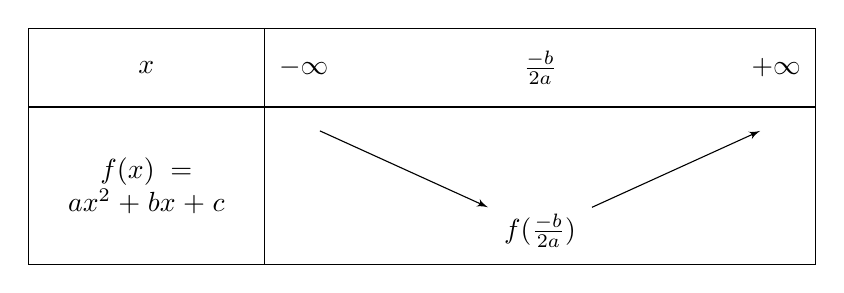
\begin{tikzpicture}
   \tkzTabInit[lgt=3]
     {$x$ / 1 , $f(x) = ax^2 +bx + c$ / 2}
     {$-\infty$,$\frac{-b}{2a}$,$+\infty$}
   \tkzTabVar
   { +/$$ ,-/$f(\frac{-b}{2a})$,+/$$}
\end{tikzpicture}


\item Si $x \leq 0$:

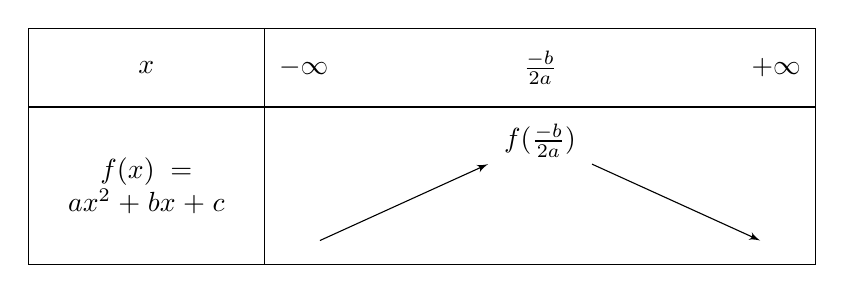
\begin{tikzpicture}
   \tkzTabInit[lgt=3]
     {$x$ / 1 , $f(x) = ax^2 +bx + c$ / 2}
     {$-\infty$,$\frac{-b}{2a}$,$+\infty$}
   \tkzTabVar
   { -/$$ ,+/$f(\frac{-b}{2a})$,-/$$}
\end{tikzpicture}
\end{itemize}


\subsection{Tableau de variations d'une fonction homographique:}
On a \[
	\Delta = \begin{vmatrix}
		a & b\\
		c & d
	\end{vmatrix}
\]
\begin{itemize}
	\item si $\Delta \geq 0$:

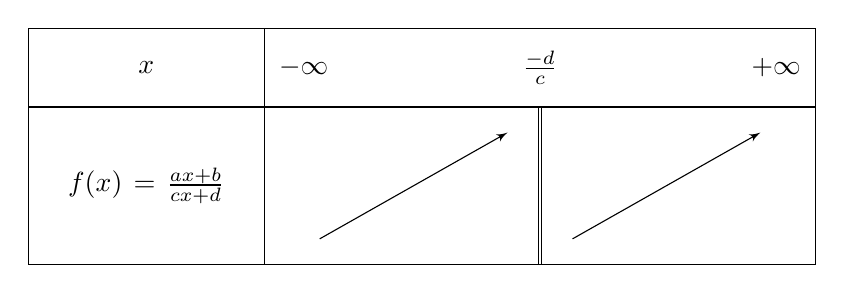
\begin{tikzpicture}
   \tkzTabInit[lgt=3]
     {$x$ / 1 , $f(x) = \frac{ax+b}{cx+d}$ / 2}
     {$-\infty$,$\frac{-d}{c}$,$+\infty$}
   \tkzTabVar
   { -/$$ ,+D-/$$,+/$$}
\end{tikzpicture}

\item si $\Delta \leq 0$:

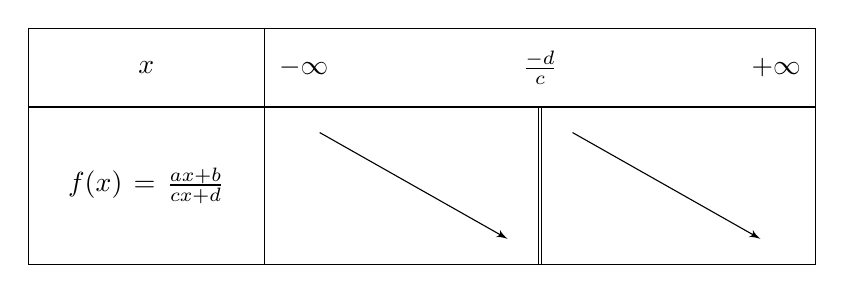
\begin{tikzpicture}
   \tkzTabInit[lgt=3]
     {$x$ / 1 , $f(x) = \frac{ax+b}{cx+d}$ / 2}
     {$-\infty$,$\frac{-d}{c}$,$+\infty$}
   \tkzTabVar
   { +/$$ ,-D+/$$,-/$$}
\end{tikzpicture}
\end{itemize}

\subsection{Tableau de variations d'une fonction $x \rightarrow \sqrt{x + a } $}
\center
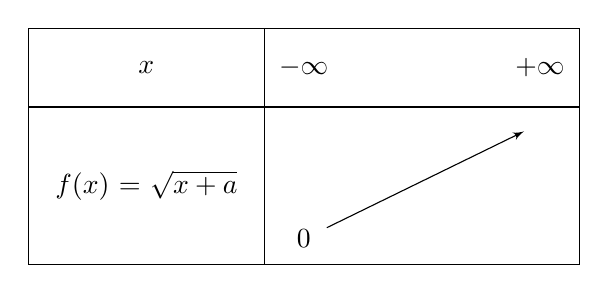
\begin{tikzpicture}
   \tkzTabInit[lgt=3]
   {$x$ / 1 , $f(x) = \sqrt{x+a}$ / 2}
     {$-\infty$,$+\infty$}
   \tkzTabVar
   { -/$0$ ,+/$$}
\end{tikzpicture}
\section{Les courbes de fonctions usuelles}
\subsection{La courbe du fonction polynome de degrée 2}
\begin{tikzpicture}
	\begin{axis}[axis lines=middle,ymin = -10,ymax=10,xmin=-10,xmax=10,domain=-15:15]
		\addplot[samples=200,color=red]{x^2 + 3*x -2};
	\end{axis}
\end{tikzpicture}

\subsection{La courbe du fonction homographique:}
\begin{tikzpicture}
	\begin{axis}[axis lines=middle,ymin = -20,ymax=20,xmin=-20,xmax=20,domain=-20:20]
	\addplot[samples=300,color=red]{(3*x +3)/(2*x)};
	\end{axis}
\end{tikzpicture}

\subsection{La courbe du fonction $x \rightarrow \sqrt{x + a }$}
\begin{tikzpicture}
	\begin{axis}[axis lines=middle,ymin = -10,ymax=10,xmin=-10,xmax=10,domain=-5:10]
		\addplot[samples=300,color=red]{sqrt(x+5)};
	\end{axis}
\end{tikzpicture}

\end{document}
